\section*{Aufgabe 1}
\subsection*{a)} 
Das Integral
\[
I_0 = \int_{-1}^1 \frac{e^x}{x}\mathrm{d}x
\]
soll numerisch integriert werden.
Dazu lässt sich das Integral umschreiben zu
\begin{align*}
I_0 &= \underset{\epsilon\rightarrow 0}\int_{\epsilon}{lim}^1\frac{e^x}{x}\mathrm{d}x + \int_{-1}^{-\epsilon}\frac{e^x}{x}\mathrm{d}x\\
&=\underset{\epsilon\rightarrow 0}{lim}\int_{\epsilon}^1\frac{e^x}{x}\mathrm{d}x - \int_{1}^{\epsilon}\frac{e^-x}{x}\mathrm{d}x\\
&=\underset{\epsilon\rightarrow 0}{lim}\int_{\epsilon}^1\frac{e^x+e^{-x}}{x}\mathrm{d}x
\end{align*}
Wird eine ONC wie etwa die Mittelpunktsregel verwendet, kann der Limes betrachtet werden, da die Funktion nicht an der Singularität ausgewertet werden muss. Es ergibt sich der Wert für das Integral zu
\[
I_0 = 2.1145017
\]
mit einem Fehler $<10^{-7}$.
\subsection*{b)}
Die Simpsonregel wird verwendet um das Integral
\[
I_1 = \int_0^{\infty} \frac{e^{-x}}{\sqrt{x}} \mathrm{d}x
\]
zu bestimmen. Um die Polstelle zu umgehen kann mithilfe einer Variablentransformation $x=u^2, \mathrm{d}x=2u\mathrm{d}u$
das Integral umschreiben zu 
\[
I_1 = \int_0^{\infty} e^{-u^2} \mathrm{d}u
\]
Da eine numerische Integration bis $\infty$ nicht möglich ist, wird bis zu einem oberen Limit $b$ integriert ($I_b$) und zur Fehlerabschätzung ebenfalls das Integral bis $b' = b+1$ bestimmt ($I_{b'}$) und die Abweichung $|I_{b'}-I_b|$ bestimmt. Das Ergebnis der Integration und die Abweichung in Abhängigkeit der oberen Grenze $b$ sind in Abb.\ref{fig:1b} und Abb.\ref{fig:1b_err} aufgetragen.
Es zeigt sich, dass bereits für eine kleines $b\approx 8$ die Abweichung mit $\mathcal{O}(10^{-16}$ vernachlässigbar klein wird und das Integral den Wert
\[
I_1 = 1.77245385
\]
annimmt.
\begin{figure}[h!]
\begin{minipage}{0.45\textwidth}
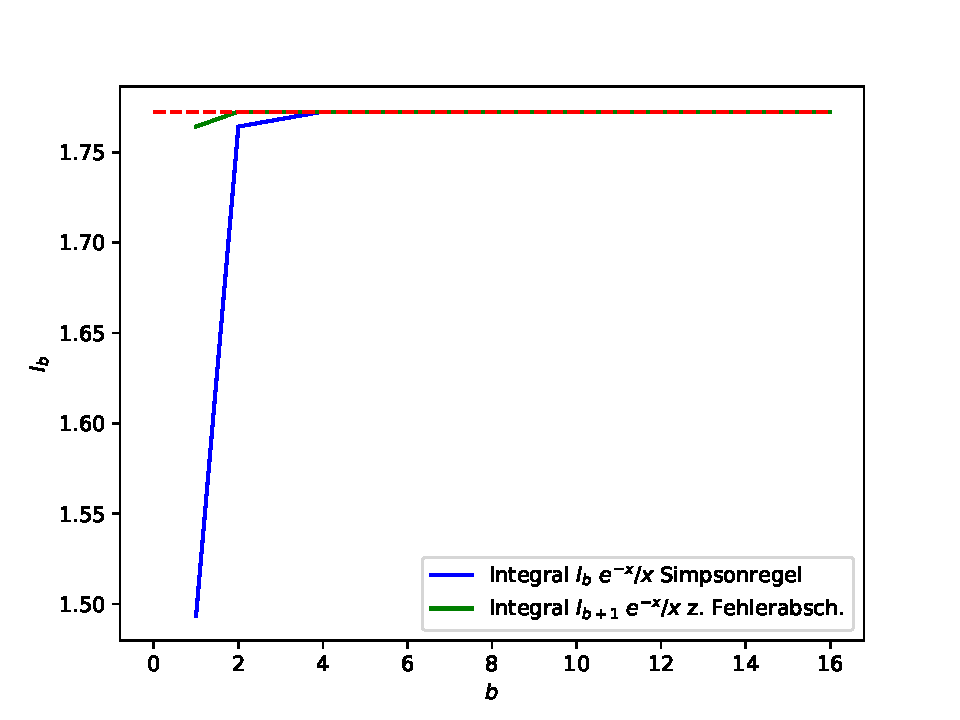
\includegraphics[width=0.9\textwidth]{A1/build/1b.pdf}
\caption{Integralberechnung von $\int_0^{\infty}\frac{e^{-x}}{\sqrt{x}}$ bis zur oberen Grenze $b$ und $b'$ mit Hilfe der Simpsonregel.}
\label{fig:1b}
\end{minipage}
\begin{minipage}{0.45\textwidth}
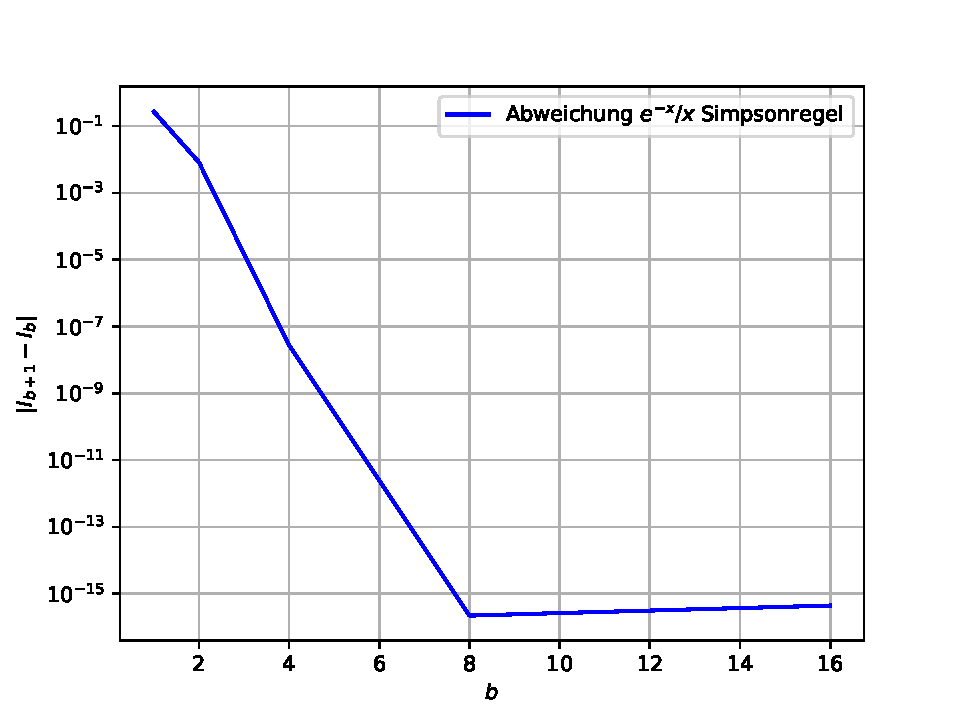
\includegraphics[width=0.9\textwidth]{A1/build/1b_err.pdf}
\caption{Fehlerabschätzung $|I_{b'}-I_b|$ von $\int_0^{\infty}\frac{e^{-x}}{\sqrt{x}}$ mit Hilfe der Simpsonregel.}
\label{fig:1b_err}
\end{minipage}
\end{figure}

\subsection*{c)}
Es soll das Integral 
\[
I_2 = \int_{-\infty}^{\infty}\frac{\sin{x}}{x}\mathrm{d}x
\]
sowohl analytisch, als auch numerisch bestimmt werden.
Zunächst lässt sich $I_2$ aus Symmetrie gründen umschreiben zu
\[
I_2 = 2\int_{0}^{\infty}\frac{\sin{x}}{x}\mathrm{d}x
\]
Nun lässt sich mit Hilfe eines Feynman-Parameters schreiben $I_2 = 2I(c=0)$ mit
\begin{equation}
I(c) = \int_0^{\infty} \frac{\sin{x}}{x}e^{-cx}\mathrm{d}x\label{eq:1}
\end{equation}
Durch Ableiten nach $c$ und anschließendes integrieren nach $x$ und $c$ erhält man so
\begin{align*}
I'(c) &= \int_0^{\infty} \sin{x}e^{-cx} \mathrm{d}x\\
&= \frac{-1}{c^2+1}\\
\Rightarrow I(c) &= -\int \frac{1}{b^2+1} = -\arctan(b) + const
\end{align*}
Die Konstante lässt sich über den Vergleich mit dem Integral I(c) aus Gleichung\eqref{eq:1} für $c\rightarrow \infty$ bestimmen zu $const = \frac{\pi}{2}$.
Damit ist
\[
I_2 = I(0) = \pi
\]
Numerisch lässt sich dies berechnen mit Hilfe der Mittelpunktsregel, wobei wieder bis zu einem Wert $b$ integriert und der Fehler abgeschätzt wird.
Das Ergebnis der Integration und die Abweichung in Abhängigkeit der oberen Grenze $b$ sind in Abb.\ref{fig:1c} und Abb.\ref{fig:1c_err} aufgetragen.
Hier dauert es deutlich länger bis die Abweichung hinreichend klein wird und sich der Wert des Integrals an
\[
I_2 = 3.14159369\]
annähert mit einer Abweichung von $\mathcal{O}(10^{-7}$.
Alternativ wäre es möglich das Integral aufzuteilen in die Grenzen von $0$ bis $1$ und $1$ bis $\infty$ und dann mit einer Variablentansformation $x = \frac{1}{y}$ für den 2. Teil das Integral umzuformen in
\[
I_2 = 2\int_{0}^{1}\frac{\sin{x}-\sin{\frac{1}{x}}}{x}\mathrm{d}x
\]
Dies führt allerdings selbst bei Verwendung von ONC zu großen Instabilitäten in der Nähe von $x=0$
\begin{figure}[h!]
\begin{minipage}{0.45\textwidth}
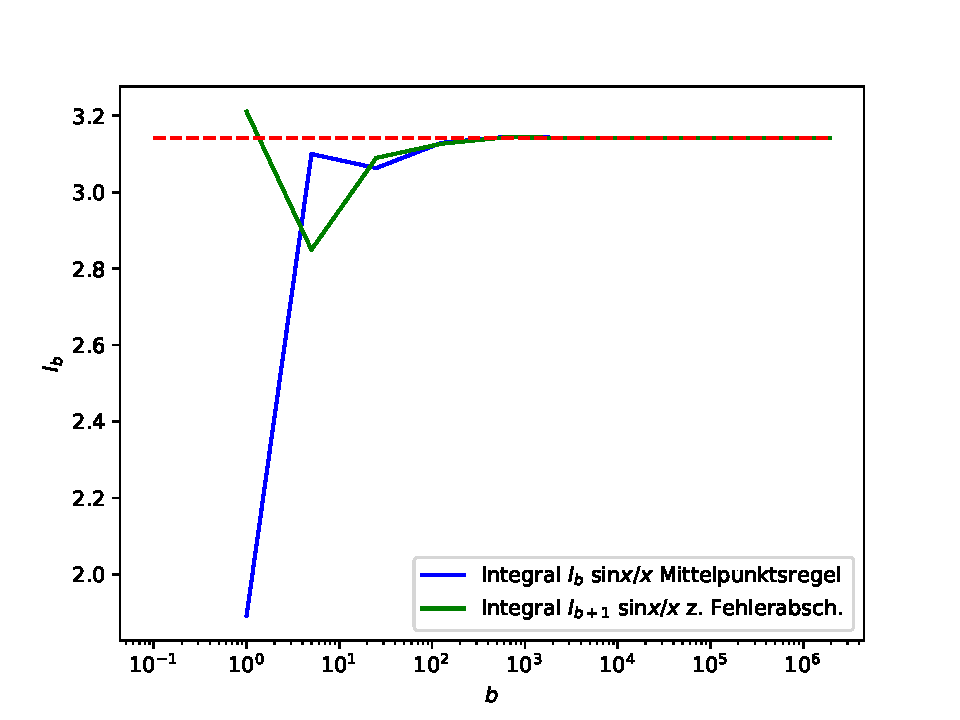
\includegraphics[width=0.9\textwidth]{A1/build/1c.pdf}
\caption{Integralberechnung von $\int_0^{\infty}\frac{\sin{x}}{\sqrt{x}}$ bis zur oberen Grenze $b$ und $b'$ mit Hilfe der Mittelpunktsregel.}
\label{fig:1c}
\end{minipage}
\begin{minipage}{0.45\textwidth}
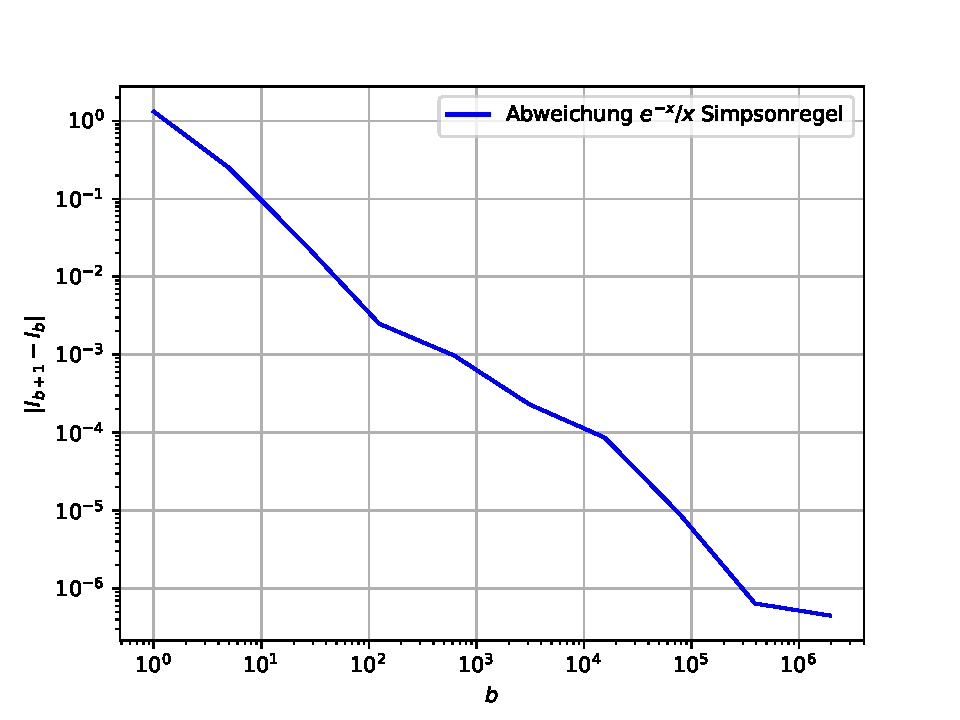
\includegraphics[width=0.9\textwidth]{A1/build/1c_err.pdf}
\caption{Fehlerabschätzung $|I_{b'}-I_b|$ von $\int_0^{\infty}\frac{\sin{x}}{\sqrt{x}}$ mit Hilfe der Mittelpunktsregel.}
\label{fig:1c_err}
\end{minipage}
\end{figure}